For correct recognition of a face the system had to do pre-processes of the
image as well as normalization of the face’s orientation and position. The
face was then analyzed with Eigenfaces to compare with the database. Some of
the steps described below used an adaptive thresholding during detection. The
decision to do this was based on the will to not dismiss images and faces in
the early pre-process steps but rather dismiss it during the comparison with
the Eigenfaces.

A brief overlook of the needed steps, which are also described below, for the detection can be seen in figure \ref{fig:overlook}.

\begin{figure}[htbp]
  \centering
  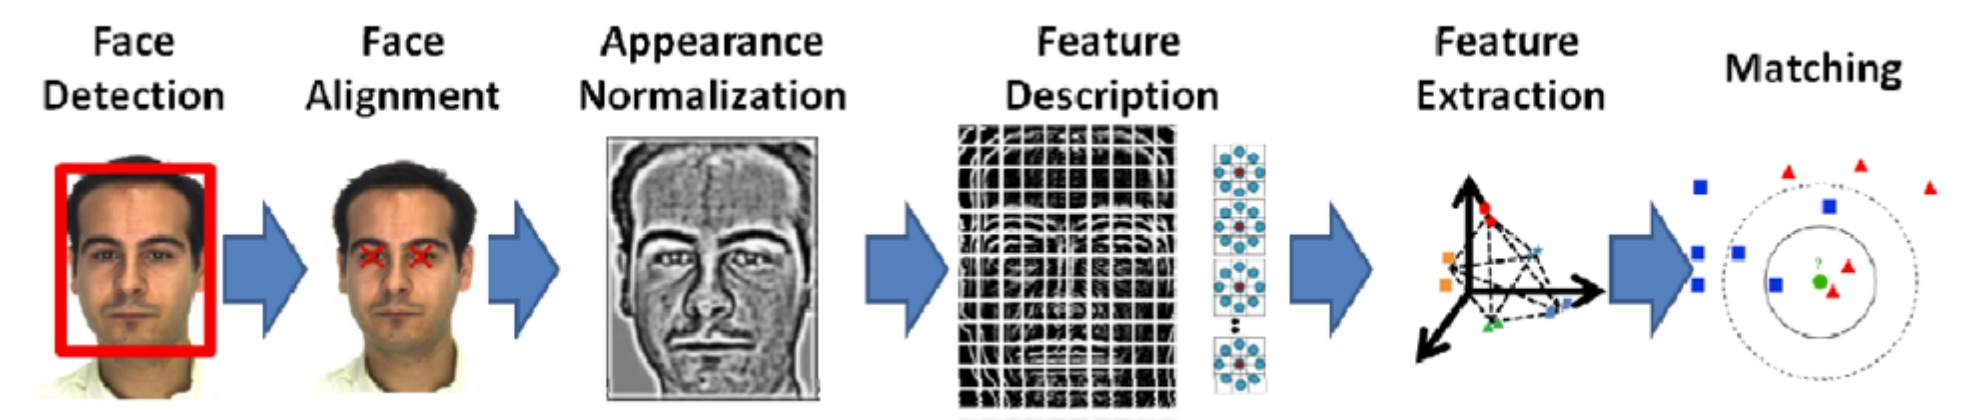
\includegraphics[width=\columnwidth]{images/process.jpg}
  \caption{Overlook of the whole face detection and recognition process.}
  \label{fig:overlook}
\end{figure}

\subsection{Lighting compensation}
Since the method of detecting a face in an image is based on color, the
potential difference in color temperature have to be eliminated. The method
used in this project was \emph{Gray world assumption}. The \emph{Gray world
assumption} method makes the assumption that the average value of the images
\emph{RGB} channels should be equal. The smallest average of the channels is
determined and then all the values in the image is scaled after this average
to eliminate any difference in white balance in images.

\subsection{Skin detection}
The first part of the recognition was to detect faces within an image. The
method used in this project was based on the implementation described by
AUTHOR2. The image’s color space was first converted from \emph{RGB} (Red,
Green, Blue) into \emph{YCbCr} (\emph{Y} being the brightness, \emph{Cb} the
blue chroma and \emph{Cr} the red chroma). The chroma channels were then
transformed into a value based on the brightness value of the pixels. This
transformation was done to be able to study the chroma values of each pixel in
a 2D space. The criteria for skin color was approximated to an ellipse in the
space of all chroma values that can be represented. The image was turned into
a binary image with only pixels within the ellipse set to white. This mask
would later be used as a mask to only show the skin areas, see figure \ref{fig:skinmask}. The last step of the skin detection was to dismiss all skin areas
except the biggest in the image and fills any holes in that area. The image
could then be cropped to this area to only contain the face part of the image.

\begin{figure}[htbp]
  \centering
  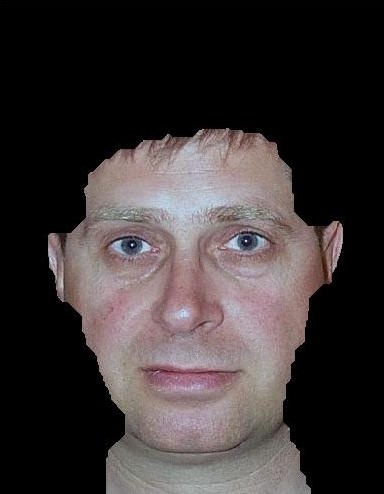
\includegraphics[width=0.6\columnwidth]{images/skinmask.jpg}
  \caption{The face mask applied to the original image.}
  \label{fig:skinmask}
\end{figure}

\subsection{Eye map}
When mapping eyes of a person a methodology presented in \cite{facedetection}
was used. The input image was converted into \emph{YCbCr} color space. This
was done since observations showed that high Cb values and low Cr values were
found around the eyes. Two different eye maps were calculated, one for the
chrominance part of the eye and one for the luminance part. To calculate an
eye map for the chrominance part equation \ref{eq:eyemapc} was used. For the
luminance part morphological operations was used to smooth out small and
irrelevant details. Equation \ref{eq:eyemapl} below was used to calculate the
luminance eye map.

\begin{equation}
  EyeMapC = \frac{1}{3}(C_b^2 + (\widetilde{C}_r)^2 + (C_b/C_r))
  \label{eq:eyemapc}
\end{equation}

\begin{equation}
  EyeMapL = \frac{Y(x, y)\oplus g_\sigma (x,y)}{Y(x, y)\ominus g_\sigma (x,y) + 1}
  \label{eq:eyemapl}
\end{equation}

To combine both eye maps elementwise multiplication was used. The combined eye
map is then dilated and masked in order to isolate the eyes. The result of the
eye detection can be seen in figure \ref{fig:eyemap}.

\begin{figure}[htbp]
  \centering
  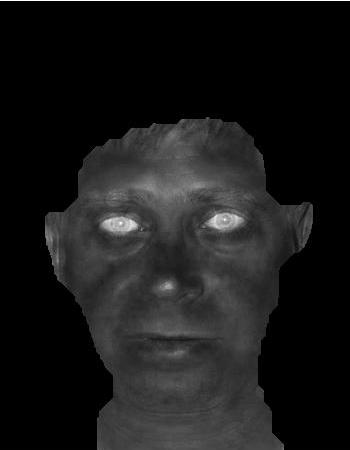
\includegraphics[width=0.6\columnwidth]{images/eye.jpg}
  \caption{The result of the eye map.}
  \label{fig:eyemap}
\end{figure}

\subsection{Mouth map}
The mouth map was calculated in a similar way to the eye map. By measuring the
different regions of the face the mouth can be detected based on the fact that
it usually has a strong red component in the facial region. The equation for
the map can be seen equations \ref{eq:mouthmap} and \ref{eq:moutheta}.
Similarly to the eye map the input image was converted into the YCbCr color
space and then processed.

\begin{equation}
  MouthMap = C_r^2 \cdot (C_r^2 - \eta \cdot C_r/C_b)^2
  \label{eq:mouthmap}
\end{equation}

\begin{equation}
  \eta = 0.95 \cdot \frac{\frac{1}{n}\sum_{(x,y)\in FG} C_r(x,y)^2}{\frac{1}{n}\sum_{(x,y)\in FG} C_r(x,y)/C_b(x,y)}
  \label{eq:moutheta}
\end{equation}

\subsection{Face alignment}
With the eye map and mouth map the important facial points could be found. The
maps were thresholded to create a binary mask. The maps were studied to find
the centroid of each white area in the mask. The different eye and mouth
candidates were then compared to each other to find the best face candidate.
The face was then warped to a normalized state with specific positions for the
eyes and mouth.

\subsection{LogAbout}
The purpose of the LogAbout method was to normalize the illumination of the
faces. This was to improve comparison in images where the the face had a wide
range of differently illuminated areas. The method was implemented using the
method suggested in \cite{logabout}. The input image was sent through a high
pass filter that can be seen in equation \ref{eq:filter}. When the filter had
been applied to the image it was transformed using a logarithmic function. The
equation used for the logarithmic function can be seen in equation
\ref{eq:logabout}.

\begin{equation}
  \begin{bmatrix}
    -1 & -1 & -1\\
    -1 & 9 & -1\\
    -1 & -1 & -1
  \end{bmatrix}
  \label{eq:filter}
\end{equation}

\begin{equation}
  g(x,y) = a + \frac{ln(f(x,y) + 1)}{b\cdot ln c}
  \label{eq:logabout}
\end{equation}

\subsection{Histogram equalization}
Similar to LogAbout, the purpose of histogram equalization was to normalize
the illumination of the faces. This method redistributes the image’s intensity
evenly throughout a larger spectrum in the histogram compared to before the
equalization. This resulted in an improved contrast in the image. \cite{histeq}
In theory, this could strengthen the distinguishing facial features of the images, but could also potentially increase the risk of failing to recognise
new features introduced to faces over time.

\subsection{Eigenfaces}
Storing and comparing a potentially large image database requires a lot of
memory, since each normalized image needs to be stored in a database and then
compared to the current image. If no action is taken to compensate for this, a
situation where the program’s memory requirements exceeds what is available is
likely to arise. To avoid this, and to lower the data size to a manageable
amount, a method called principal component analysis (PCA) was used. In
practice the number of dimensions in the high-dimensional dataset, that the
image database constitutes, is reduced.

This dimension reduction was performed by focusing on the difference between
the images. Correlated variables are not interesting when the aim is to
distinguish variance and make decisions upon differences. What was interesting
however was the uncorrelated variables. By calculating the mean image out of
all images in the database and subtracting this mean from a candidate image,
the unique features of the image were highlighted. This was used to calculate
the covariance matrices for the images, which in turn was used to calculate
eigenvalues and eigenvectors. These eigenvalues and eigenvectors were then
used to match candidate images with the images in the database. The resulting images can be seen in figure \ref{fig:eigen}.

\begin{figure}[htbp]
  \centering
  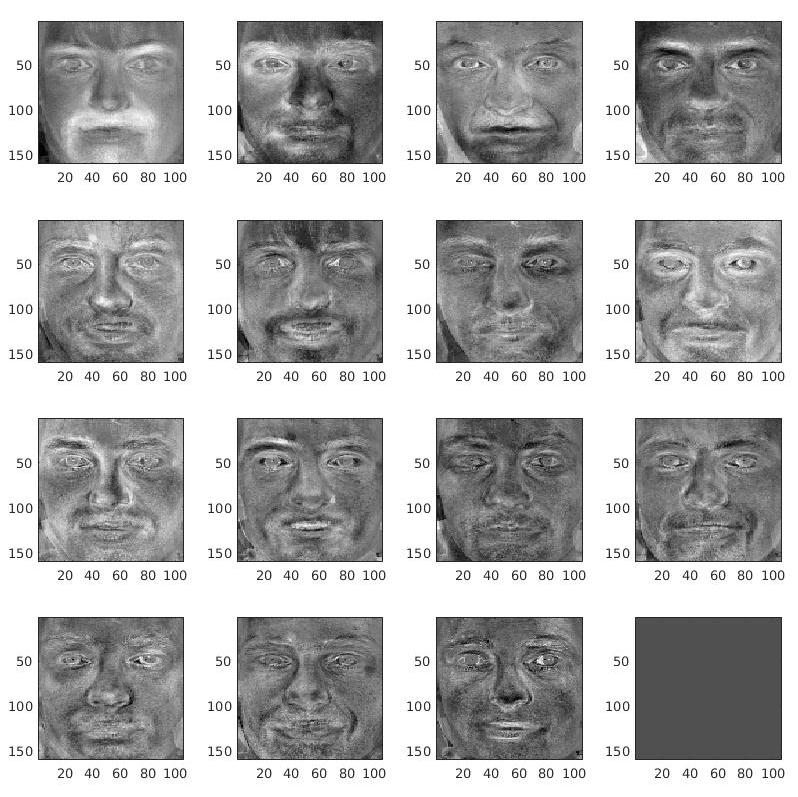
\includegraphics[width=\columnwidth]{images/eigen.jpg}
  \caption{Eigenfaces in the database.}
  \label{fig:eigen}
\end{figure}

\subsection{False negatives and false positives}
Naturally, the program errors in some cases. There are two cases that deserves
to be mentioned here; false negatives and false positives. False negatives are
when the system does not match a face it should know. This can occur because
the image is discarded in the thresholding of the summed error, when the
system isn’t satisfyingly certain of the result. False positives is when the
program simply guesses wrong, but with such a certainty that it passes the
thresholding that should stop it. The result amount of false negatives and
false positives can be studied with two rates, \emph{false rejection rate}
(FRR) and \emph{false acceptance rate} (FAR). FRR measures the rate in which a
face in the database is not recognized and rejected, while FAR measures the
rate of an unknown face mismatched with a face in the database.
